\documentclass[dvipdfmx]{jarticle}
\usepackage{amsmath,amssymb,amsfonts,amsthm}
\usepackage[dvipdfmx]{graphicx}
\usepackage{tikz}
\usetikzlibrary{positioning, intersections, calc, arrows.meta, math, through}
\usepackage{tcolorbox}
\tcbuselibrary{theorems,breakable}
\usepackage{enumerate}
\usepackage{mathtools}
\usepackage{otf}
\usepackage{xspace}
\usepackage{newpxtext}
\usepackage[utf8]{inputenc} %中国語コンパイル環境-cjkホットショット
\usepackage{CJKutf8} %中国語コンパイル環境
\usepackage{okumacro} %漢字ruby
\usetikzlibrary{calc}
\renewcommand{\abstractname}{注意事項}
\newtagform{textbf}[	extbf]{[}{]}
\usetagform{textbf}
\newcommand*{\ie}{\textbf{\textit{i.e.}}\@\xspace}
\renewcommand{\qedsymbol}{$\blacksquare$}
\newtcbtheorem[]{reidai}{例題}
{fonttitle=\gtfamily\sffamily\bfseries\upshape\large,
colframe=black,colback=black!15!white,
rightrule=1pt,leftrule=1pt,bottomrule=2pt,
colbacktitle=black,theorem style=standard,breakable,arc=10pt}
{tha}
\renewcommand{\thefootnote}{\arabic{footnote}}
\newtheoremstyle{mystyle}%
  {}%                      % 上部スペース
  {}%                      % 下部スペース
  {}%                      % 本文フォント
  {}%                      % 1行目のインデント量
  {\bfseries}%             % 見出しフォント
  :%                       % 見出し後の句読点
  { }%                     % 見出し後のスペース
  {\thmname{#1}\thmnumber{ #2}\thmnote{ (#3)}}
\theoremstyle{mystyle}
% \setcounter{section}{0}
% \stepcounter{section}
% セクションカウンターを使用するが、表示はしない新しいセクションコマンドを作成
\newtheorem{dfn}{\texttt{Def.}}[section]
\newtheorem{exm}[dfn]{\texttt{Ex.}}
\newtheorem{prop}[dfn]{\texttt{Prop.}}
\newtheorem{lem}[dfn]{\texttt{Lem.}}
\newtheorem{thm}[dfn]{\texttt{Thm.}}
\newtheorem{cor}[dfn]{\texttt{Cor.}}
\newtheorem{rem}[dfn]{\texttt{Rem.}}
\newtheorem{fact}[dfn]{\texttt{Fact}}
\renewcommand{\qedsymbol}{$\blacksquare$}
\usepackage{lipsum} % 用于生成示例文本
\usepackage{float} % 强制浮动
\usepackage{tikz} % 用于定位
%排版
\newcommand{\kai}%解答
{\noindent
\begin{tikzpicture}[scale=0.2, baseline=2.8pt]
\draw (3.3,1) node{\large\textgt{解 答}};
\draw[thick, rounded corners=3pt,] (0,0)--(6.5,0)--(6.5,2.2)--(0,2.2)--cycle;
\end{tikzpicture};}
\newcommand{\shomei}%証明
{\noindent
\begin{tikzpicture}[scale=0.2, baseline=2.8pt]
\draw (3.3,1) node{\textgt{証 明}};
\draw[double,thick,rounded corners=3pt,] (0,0)--(6.5,0)--(6.5,2.2)--(0,2.2)--cycle;
\end{tikzpicture};}
%補足
\newcommand{\hosoku}{\noindent
\begin{tikzpicture}[scale=0.2, baseline=2.8pt]
\draw (6,1) node{\large\textgt{補足}};
\fill (0,1)--(1,0)--(2,1)--(1,2)--cycle;
\fill[gray] (1,1)--(2,0)--(3,1)--(2,2)--cycle;
\fill (2,1)--(3,0)--(4,1)--(3,2)--cycle;
\fill (10,1)--(11,0)--(12,1)--(11,2)--cycle;
\fill[gray] (9,1)--(10,0)--(11,1)--(10,2)--cycle;
\fill (8,1)--(9,0)--(10,1)--(9,2)--cycle;
\end{tikzpicture};}
%注意
\newcommand{\chui}{\noindent
\begin{tikzpicture}[scale=0.2, baseline=2.8pt]
\fill (0,0)--(6.5,0)--(6.5,2.2)--(0,2.2);
\draw (3.3,1) node[white]{\large\textgt{注意!}};
\draw[thick] (0,0)--(6.5,0)--(6.5,2.2)--(0,2.2)--cycle;
\end{tikzpicture};}
\title{\vspace{-3cm}\textbf{\huge 円周角の定理とその証明}}  %タイトル
\author{\empty}  %著者名
\date{}  %日付
\begin{document}
\maketitle
%\vspace{-0.4cm}
%\begin{figure}[H]
%\centering
%\begin{tikzpicture}[remember picture, overlay]
%   \node[anchor=north east] at (current page.north east) {%
%        \includegraphics[width=2cm]{pics/qr.png} % 修正图片地址
%    };
%    \node[anchor=north east, yshift=-2cm] at (current page.north east) {デジタル版はここ};
%\end{tikzpicture}
%\label{fig:my_label}
%\end{figure}
%\begin{abstract} %概要
  %注意事項
%\end{abstract}
%\begin{reidai}{2次方程式}{解答}
%\end{reidai}
%\begin{proof}
%\end{proof}
\section{\textbf{円周角の定理}}
\begin{dfn}[円周角の定理]
\item[1.] {\color{blue}{中心角}} は {\color{red}{円周角}} の2倍である。
\item[2.] 同じ弧に対する円周角は全て等しい。\\

\begin{tikzpicture}[thick, scale=3]

% Draw the main circle
\draw[very thick] (0,0) circle(1);

% Points on circumference
\coordinate (A) at (-0.7,-0.7);
\coordinate (B) at (0.7,-0.7);
\coordinate (C) at (0,1);

% Intersection points on circle - moved down slightly
\coordinate (D) at (-0.22,0.97);
\coordinate (E) at (0.22,0.97);
% Draw the thick base
\draw[very thick] (A) -- (B);

% Draw perimeter triangle legs and diagonals
\draw[very thick] (A) -- (D) -- (B);
\draw[very thick] (A) -- (E) -- (B);

% The upper "apex" to right and left vertex
\draw[very thick] (D) -- (E);

% Red circles at upper points - moved down
% Intersection points on circle - moved down slightly
\coordinate (D) at (-0.22,0.8);circle(0.04);
\fill[red] (D) circle(0.04);
\coordinate (E) at (0.22,0.8); circle(0.04);
\fill[red] (E) circle(0.04);

% Draw the center point
\coordinate (O) at (0,0);
\fill (O) circle(0.025);

% Purple square below circle center
\filldraw[fill=purple!60!blue, draw=purple!80!blue] (-0.04,-0.12) rectangle (0.04,-0.04);

% Dashed lines for central angle
\draw[thick,dashed] (O) -- (A);
\draw[thick,dashed] (O) -- (B);

% Purple label "中心角" near bottom
\node[align=center,color=purple,font=\bfseries,scale=1.1] at (0,-0.35) {中心角};

% Top right: "円周角" in red
\node[align=center,color=red,font=\bfseries,scale=1.2, anchor=west] at (0.6,0.95) {円周角};
\end{tikzpicture}
\end{dfn}
\section{\textbf{円周角の定理の証明}}
\begin{proof}
  円周角の定理1:「中心角=円周角の2倍」を証明する。\ie つまり、円周角を$\angle ACB$、円の中心を$O$として、$\angle AOB = 2\angle ACB$を証明します。\\

\noindent
三角形$ABC$の内側に$O$があるとき\\

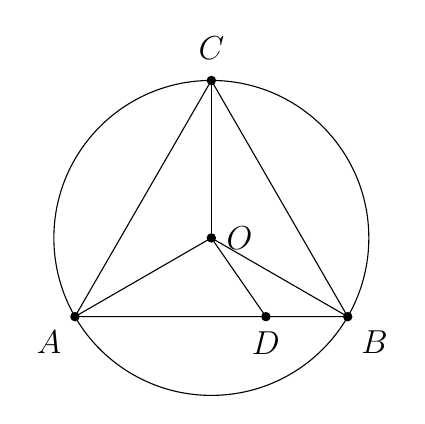
\begin{tikzpicture}[scale=2]
    % 圆
    \coordinate (O) at (0,0);
    \def\radius{1}
    \draw (O) circle (\radius);

    % 圆周上的点
    \coordinate (A) at ({\radius*cos(210)}, {\radius*sin(210)});
    \coordinate (B) at ({\radius*cos(330)}, {\radius*sin(330)});
    \coordinate (C) at ({\radius*cos(90)}, {\radius*sin(90)});

    % D点在AB上偏右
    \coordinate (D) at ($(A)!0.7!(B)$);

    % 线段
    \draw (A) -- (B) -- (C) -- cycle;
    \draw (O) -- (A);
    \draw (O) -- (B);
    \draw (O) -- (C);
    \draw (O) -- (D);

    % 标记点
    \fill (O) circle (0.03);
    \fill (A) circle (0.03);
    \fill (B) circle (0.03);
    \fill (C) circle (0.03);
    \fill (D) circle (0.03);

    % 文字
    \node[font=\large, below left=2pt] at (A) {$A$};
    \node[font=\large, below right=2pt] at (B) {$B$};
    \node[font=\large, above=4pt] at (C) {$C$};
    \node[font=\large, below=2pt] at (D) {$D$};
    \node[font=\large, right=2pt] at (O) {$O$};
\end{tikzpicture}

\end{proof}
\end{document}